\chapter{相关研究工作}
本章主要论述高性能互连网络设计的相关背景知识。
首先介绍了物理器件对新型高性能互连网络的影响,
之后介绍了典型的高性能互连网络拓扑结构和路由算法。

\section{物理器件对高性能互连网络的影响}
传统的高性能互连网络拓扑大致分为两类
,一类是以$k-ary$ $n-fly$蝶形网络为代表的间接网络,
如图\ref{butterfly}所示。
$k-ary$ $n-fly$结构中,节点度数为$2k$,采用单向链路,
网络直径为$n-1$,网络规模为$k^n$。
一类是以$k-ary$ $n-cube$网络为代表的直接网络,
如图\ref{torus} 所示。
$k-ary$ $n-cube$结构中,节点度数为$2n$,采用双向链路,
网络直径为$n(\lfloor\frac{k}{2}\rfloor)$,网络规模为$k^n$。
当$k=2$时,$k-ary$ $n-cube$结构就是经典的超立方体(Hypercube)结构,
是第一代高性能计算机的主要拓扑结构。
如Intel iPSC/2\upcite{ipsc2}、 NCUBE/10\upcite{ncube}、
SGI Origin 2000\upcite{sgi2000} 等系统均采用了Hypercube结构,
因为其具有正则性、对称性、强容错性以及可嵌入性等特点。
当$k=n$时,$k-ary$ $n-fly$结构和$k-ary$ $n-cube$结构规模一样,
节点度数一样,但是$k-ary$ $n-cube$结构的网络直径大约是
$k-ary$ $n-fly$结构的$\frac{k}{2}$倍。
$k-ary$ $n-fly$ 结构拥有更小的网络直径,
但是,路径唯一性及负载不均衡是限制其发展的主要原因。

\begin{figure}[htp]
  \centering
   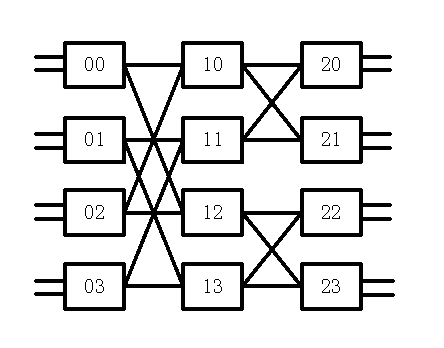
\includegraphics[width=.48\textwidth,height=.38\textwidth]{Visio-butterfly.eps}
    \caption{$k-ary$ $n-fly$结构}
    \label{butterfly}
\end{figure}

\begin{figure}[htp]
  \centering
   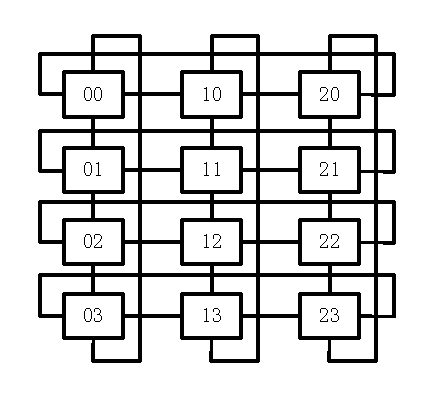
\includegraphics[width=.44\textwidth,height=.38\textwidth]{Visio-torus.eps}
      \caption{$k-ary$ $n-cube$结构}
      \label{torus}
\end{figure}

上世纪90年代,路由芯片引脚带宽被限制在10Gb/s的水平上,
路由芯片也因此端口数受限制。
传统的高性能互连网络只能采用低节点度的拓扑结构。
随着半导体和集成电路的发展,路由芯片的引脚带宽增加,芯片端口数也随之增加。
如Cray 公司推出的端口数为64的YARC路由芯片
\upcite{yarc}\upcite{blackwindow}、2010年HOTI
会议上提出的48端口Gemini芯片\upcite{cascade}、
2015年HOTI会议上提出48端口的Intel Omni-Path芯片\upcite{omni}以及
Mellanox 公司最新推出的Quantum 200G HDR InfiniBand Switch\upcite{quantum}。
相比使用较少宽带宽端口的路由芯片搭建高性能互连网络,
拥有更多窄带宽端口的路由芯片可以降低网络的延迟和成本开销。
根据Kim的推导,低负载下报文的网络延迟为$T=T_h+T_s=Ht_r+L/b$,
$H$是报文的跳步数,$t_r$是每一跳经过路由器的延迟,$L$是报文的长度,
$b$则是链路的带宽。
在规模为$N$的网络中,若使用端口数为$k$的路由芯片($k$ 个输入通道$k$ 个输出通道),
其跳步数最少为$2log_kN$。
若芯片的总带宽为$B$,则$b=B/2k$。
那么网络延迟为$T=2t_rlog_kN+2L/B$,对$k$求导,
当$dT/dk=0$时可得到网络延迟$T$的极值则$klog^2k=\frac{Bt_rlogN}{L}$。
随着网络规模增加,路由芯片的最佳端口数也随之增加。
因此,基于高阶路由器设计的高性能互连网络成为高性能互连网络设计的主流趋势。
相关拓扑结构相继被提出,
如Flattened Butterlfy \upcite{Flattenedbutterfly}、Dragonfly \upcite{dragonfly}、
HyperX \upcite{hyperx}等。
相比传统的高性能互连网络拓扑结构,
基于高阶路由器设计的高性能互连网络拓扑结构不仅可以支持更大的规模降低网络直径,
还可以减少路由器的数量。
Kim曾预测,未来几年内将会出现数百个端口的路由芯片,
2010年单芯片的总带宽将突破20Tbps\upcite{yarc}\upcite{blackwindow}。
但是,实际上目前最新的商用芯片总带宽只能达到16Tbps\upcite{quantum}。
随着E级计算时代的到来,规模需求增大,性能要求提高,
但是路由芯片发展远远没有达到预期的目标。
目前的高性能互连网络在高阶路由芯片端口数的限制下面临巨大挑战。
如何利用当前商用路由芯片搭建E级计算系统成为高性能互连网络的关键问题。

光纤技术的发展促进了高性能互连网络在实际系统中的部署。
大规模低直径的新型高性能互连网络相比传统的高性能互连网络,
拥有更多的全局链路以降低网络直径。
对全局链路采用光纤部署,不仅在性能上有优势,而且在能耗上独立于物理长度。
除此之外,10米以内的链路,采用光纤的成本相比电缆的成本要高,
而10米以上的链路,
则采用电缆的成本要比光纤的高\upcite{dragonfly}。
因此,为了降低系统成本,
Dragonfly结构在保证网络直径低的前提下,
每个超级节点只引出一条全局链路连接相邻超级节点\upcite{dragonfly}。
但是,E级计算系统的应用负载复杂多样,
除了对网络结构的局部性有要求外,全局通信将更加频繁,
如Dragonfly拓扑若只保证超级节点间
只有一条全局链路已不能满足应用负载的需求。
从边缘可插拔光纤收发器到主板集成光模块的转变\upcite{BOA},
多芯光纤(Multicore Fiber)\upcite{MCF}的出现将
给高性能互连网络设计又带来了新的契机,
这给增加实际部署中机柜间通信带宽提供了重要机会。
多芯光纤,如图\ref{mcf}所示,实际上就是一条光缆里有多个纤芯的光缆,
可以通过分线器分成多个单芯光纤。
一条多芯光纤相比同等纤芯数的一捆单芯光纤,
不仅成本上更加经济,而且维护上更加容易。
因此,如何在高性能互连网络中使用多芯光纤,
从而有效提升全局通信带宽并保证网络性能和可扩展性是使用多芯光纤搭建
E级计算系统的关键问题。

\begin{figure}[htp]
  \centering
    
\includegraphics[width=.48\textwidth,height=.38\textwidth]{Visio-SCF.eps}
    \caption{单芯光纤}
    \label{scf}
\end{figure}

\begin{figure}[htp]
  \centering
    
\includegraphics[width=.48\textwidth,height=.38\textwidth]{Visio-MCF.eps}
      \caption{多芯光纤}
       \label{mcf}
\end{figure}

\section{高性能互连网络新型拓扑结构}

\subsection{Fat tree}
Fat tree\upcite{fattree}是最早的大规模低直径高性能互连网络拓扑结构。
国防科技大学自主研制的天河一号和天河二号高性能计算机均采用的是Fat tree结构。
其是一个灵活性和扩展性都较优的拓扑结构,
最大的特点在于随着网络规模的增加,二分带宽也随之等规模增加。
其可以看成是两个$k-ary$ $n-fly$结构合并而成,
如图\ref{fattree}所示由两个图\ref{butterfly}合并而成,采用双向链路。
两个蝶形结构分别起到负载均衡和控制输入输出的作用,
因此,Fat tree可以有效避免蝶形网络路径唯一和负载不均衡等缺点
并继承了蝶形结构网络直径低的优点。
Fat tree的节点度数为$2k$,网络直径为$2(n-1)$,
网络规模$2k^n$,且需要$(2n-1)k^{n-1}$个路由器。

\begin{figure}[htp]
  \centering
    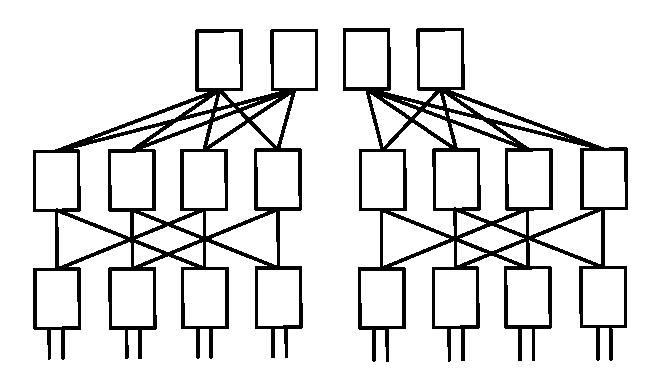
\includegraphics[width=.48\textwidth,height=.38\textwidth]{Visio-fattree.eps}
    \caption{Fat tree结构}
     \label{fattree}
\end{figure}

\subsection{Flattened Butterlfy}

Flattened Butterfly\upcite{Flattenedbutterfly}是2007年Kim等人
在ISCA会议上提出的一个性价比高的高阶互连网络。
Flattened Butterfly结构充分利用高阶路由器提供丰富的链路特性,
使得$k-ary$ $n-cube$结构中每一维上的路由节点都是全互连,
则节点度为$(n+1)(k-1)+1$,网络直径为$n$,网络规模为$k^{n+1}$。
Flattened Butterfly利用高阶路由器有效解决$k-ary$ $n-cube$结构网络直径长的问题。
同时,Flattened Butterfly利用高阶路由器合并$k-ary$ $n-fly$结构中的路由器,
有效降低路由器的数量。
如图\ref{flattenedbutterfly}所示,图左是$k-ary$ $n-fly$结构,
图右是合并了蝶形网络中每一层的路由器的Flattened Butterfly。
而且,当搭建同样规模和同样直径的网络时,
Flattened Butterfly 可以节省Fat tree近一半的链路。

\begin{figure}[htp]
  \centering
    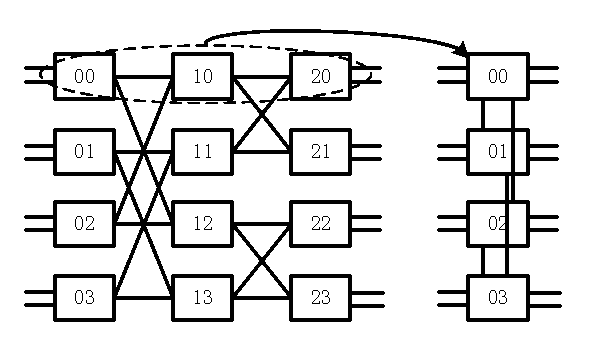
\includegraphics[width=.56\textwidth,height=.35\textwidth]{Visio-flattenedbutterfly.eps}
    \caption{Flattened Butterfly结构}
    \label{flattenedbutterfly}
\end{figure}

2009年SC会议上提出的HyperX\upcite{hyperx}
结构实际上是基于Flattened Butterfly结构的扩展结构,
是一个可以灵活配置的高阶互连网络。
HyperX同样是一个$k-ary$ $n-cube$结构,
但是每一维上的$k$值可以取不同值,
而且每个路由节点所连接的终端数以及每一维上的链路带宽都可以随意配比。
这类可灵活配置的拓扑结构更适合实际系统的需求,
不仅是在网络规模上和性能需求上还是在能耗成本开销上。
Hypercube和Flattened Butterfly都是HyperX的特例。

\subsection{Dragonfly}

Dragonfly\upcite{dragonfly}结构是一个有标志意义的高阶互连网络,
也是大规模低直经高性能互连网络的典型代表。
相比低阶互连网络,高阶互连网络拥有更多的全局链路,使用更多的长缆线。
为了解决高阶互连网络长缆线成本开销的问题,Dragonfly利用层次化的结构有效
减少了全局链路的数量并同时提供了较大的网络规模和较低的网络直径。

Dragonfly具体构造是将$a$个高阶路由器通过全互连的方式相连成虚拟的更高阶超级节点,
则每个路由节点引出$a-1$条本地链路连接同一个超级节点内的其他路由节点,
如图\ref{dragonfly}所示的虚拟框。每个路由器引出$h$条全局链路
链接其他超级节点内的路由节点。
在全局网络中,虚拟的更高阶超级节点两两之间至少一条链路相连,
如图\ref{dragonfly}所示的虚拟框之间的互连。
通过在不同层次的网络中采用全互连结构,使得Dragonfly的网络直径只有3。
相比同样规模和同样节点度数的Flattened Butterfly结构,
Dragonfly结构可以节省近一半的全局链路。

\begin{figure}[htp]
  \centering
    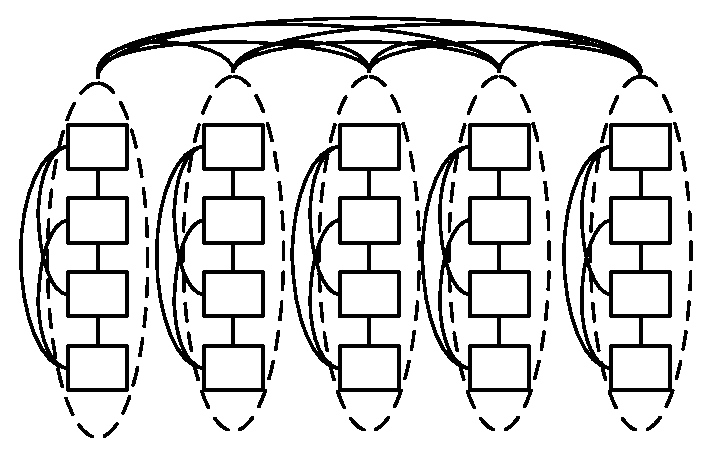
\includegraphics[width=.56\textwidth,height=.35\textwidth]{Visio-dragonfly.eps}
    \caption{Dragonfly结构}
       \label{dragonfly}
\end{figure}

在2017年HiPINEB会议上提出的Dragonfly+\upcite{Dragonfly+}
拓扑结构是在Dragonfly结构的基础上进行扩展优化,
使用直径为2的树形结构替代Dragonfly结构超级节点内的全互连网络,
同时保持网络直径为3,
如图\ref{dragonfly+}所示的结构替代图\ref{dragonfly}中的超级节点。
在使用相同端口数的路由芯片搭建网络的条件下,
Dragonfly+结构可以支持近4倍规模的Dragonfly结构。

\begin{figure}[htp]
  \centering
    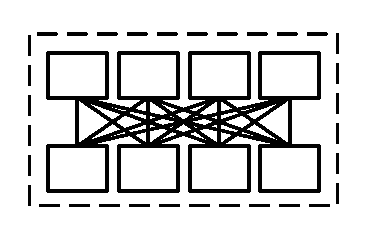
\includegraphics[width=.48\textwidth]{Visio-dragonfly+.eps}
    \caption{Dragonfly+结构中超级节点模块}
    \label{dragonfly+}
\end{figure}

\subsection{Slim Fly}
Slim Fly\upcite{slimfly}是一个近似最优拓扑结构的高性能互连网络结构,
在直径为2的约束下,
使用尽可能少的路由器端口数构造更大规模的拓扑结构。
Slim Fly结构是继Dragonfly结构之后又一个标志性拓扑结构,
其利用代数图论的构造方法,
满足了低直径大规模的要求,
而且其在二分带宽和成本能耗以及容错性上都展现了较优的性能。

Slim Fly实际上采用了代数图论里的MMS图\upcite{MMS}。
MMS图是一个高对称性的结构,由两个子图构成,
每个子图内由同样数目的子组组成,每个子组内的节点数相同。
Slim Fly的构造取决于素数幂$q$,$q$满足
$q=4w+\delta$且$\delta \in \{-1,0,1\}$。
每个路由器引出$q-\delta$条链路连接同一个子组内的路由节点,
引出$q$条链路分别连接另一个子图$q$个子组的路由节点。
Slim Fly中的每个路由节点编码为$(a,x,y)$,
其中$a\in \{0,1\}$来标识子图的编号,
以及$x,y\in\mathds{F}_q$则分别标识在所在子图中子组的编号和
所在子组中路由节点位置的编号,
如图\ref{slimflyone}所示。Slim Fly的具体连接关系满足:

当且仅当$y-y' \in X$,路由节点$(0,x,y)$与路由节点$(0,x,y')$相连。
当且仅当$y-y' \in X'$,路由节点$(1,x,y)$与路由节点$(1,x,y')$相连。
当且仅当$y=x'x+y'$,路由节点$(0,x,y)$与$(1,x',y')$相连。

其中,集合$X$和$X'$是有限域$\mathds{F}_q$的生成集合\upcite{MMS}\upcite{GRMMS}。
集合$X$和$X'$通过有限域$\mathds{F}_q$的生成元$\xi$ 构成,
如下面等式\ref{equ:generator-sets0}和\ref{equ:generator-sets1}所示。

\begin{equation}\label{equ:generator-sets0}
  X=
  \begin{cases}
    \{1,\xi^2,\ldots,\xi^{q-3}\}& q=4 \ell+1 \\
    \{1,\xi^2,\xi^4,\ldots, \xi^{2\ell-2},\\\xi^{2\ell-1},\xi^{2\ell+1},\ldots, \xi^{4\ell-3}\} & q=4 \ell-1 \\
    \{1,\xi^2,\ldots,\xi^{4l-2}\} & q=4 \ell
  \end{cases}
\end{equation}
\begin{equation}\label{equ:generator-sets1}
  X'=
  \begin{cases}
    \{\xi,\xi^3,\ldots,\xi^{q-2}\} & q=4 \ell+1 \\
    \{\xi,\xi^3,\xi^5,\ldots,\xi^{2\ell-1}, \\\xi^{2\ell},\ldots,\xi^{4\ell-4},\xi^{4\ell-2}\}\ \ \ \  & q=4 \ell-1 \\
    \{\xi,\xi^3,\ldots,\xi^{4l-1}\} & q=4 \ell
  \end{cases}
\end{equation}

在实际物理部署中,Slim Fly 可以部署成全局网络是一个全互连网络。
分别位于相邻子图的两个子组封装成一个机柜,
那么任意两个机柜之间都有$2q$条链路,
如图\ref{slimfly}所示。

\begin{figure}[htp]
  \centering
    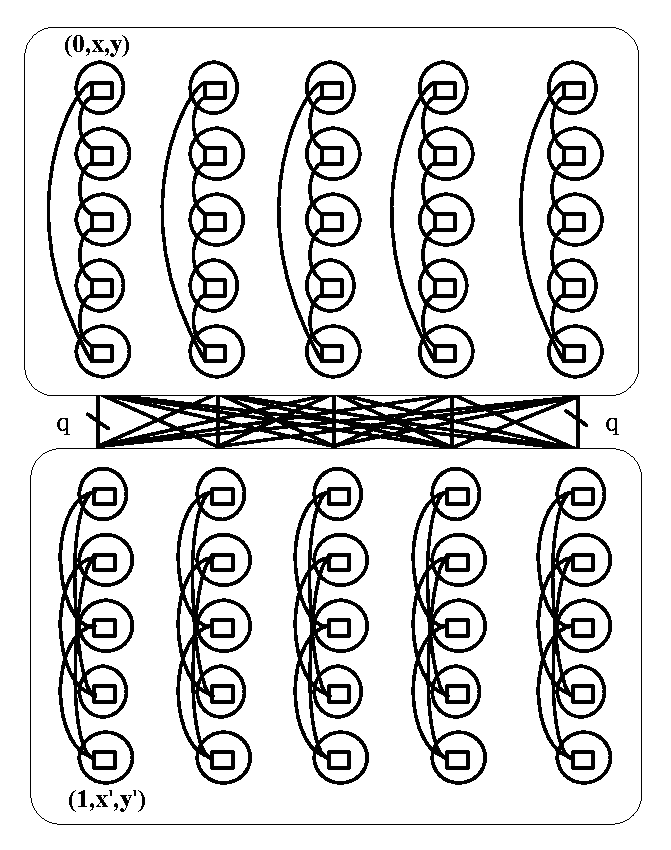
\includegraphics[width=.6\textwidth]{Visio-Slimfly_between.eps}
    \caption{Slim Fly结构}
    \label{slimflyone}
\end{figure}

\begin{figure}[htp]
  \centering
    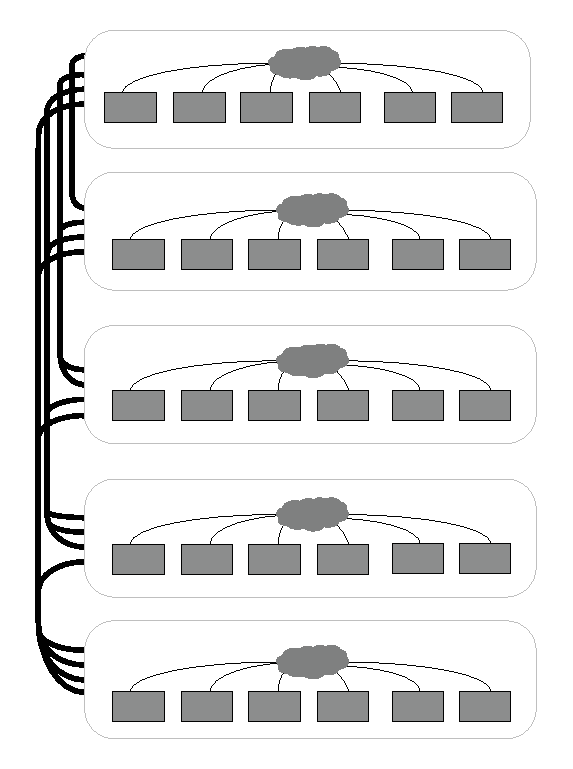
\includegraphics[width=.3\textwidth,height=.5\textwidth]{Visio-Slimfly.eps}
    \caption{Slim Fly结构的全局网络}
    \label{slimfly}
\end{figure}

在2015的SC会议上,两种网络直径为2的间接拓扑结构
OFT(two-level Orthogonal Fat-Trees)和MLFM(Multi-Layer Full-Mesh)
被提出\upcite{costeffective2},
分别如图\ref{oft}和\ref{mlmf} 所示。
在相同条件下,OFT相比Slim Fly和MLMF可以构造近似2倍规模的网络,
MLMF的可扩展性跟Slim Fly一样。
这三种拓扑结构的相同点就是平均每个终端都是消耗3个路由器端口和2条链路。

\begin{figure}[htp]
  \centering
    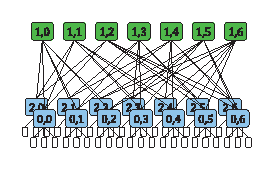
\includegraphics[width=.6\textwidth]{oft.eps}
    \caption{OFT结构\upcite{costeffective2}}
    \label{oft}
\end{figure}

\begin{figure}[htp]
  \centering
    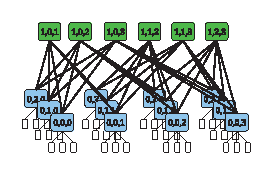
\includegraphics[width=.6\textwidth]{mlmf.eps}
    \caption{MLMF结构\upcite{costeffective2}}
    \label{mlmf}
\end{figure}

\subsection{随机拓扑}

除了前面介绍的规则拓扑外,
随机拓扑也是高性能互连网络新型拓扑结构的一个重要类型。
最早是在数据中心网络中提出使用小世界网络\upcite{smallworld}构造系统。
通过在规则拓扑结构上添加随机链路构造出具有小世界网络特性的随机网络,
如图\ref{sw2d} 所示在2维Torus结构上添加随机链路的小世界网络。
在约束节点度情况下,具有小世界网络特性的网络
不仅可以拥有较短的网络直径而且具备较高带宽和较短平均最短路径等特性。
Singla等人提出将Jellyfish\upcite{Jellyfish}
运用在top-of-rack(ToR)交换机之间。
Jellyfish是一个绑定节点度的随机图拓扑结构,
不仅可以支持任意规模,而且相比同样配置的Fat tree,
可以支持更多的节点并提供至少一样的带宽。
Valadarsky等人指出当前最新的拓扑结构,如Slim Fly和Jellyfish,
都是expander图\upcite{xpander}。
但是,在性能上这些结构还不能近似最优并在扩展上和部署上都存在困难。
因此,提出Xpander结构\upcite{xpander},不仅提供近似最优的性能,
而且在部署上切实可行。
Xpander是一个灵活扩展的拓扑结构,
每个节点表示一个ToR交换机,每个节点有$d$个端口连接其他ToR交换机。
每次扩展以$d+1$个节点的全互连图为单位进行扩展。
通常情况下,Xpander结构都是通过翻倍的方式扩展,
但是Xpander也支持线性扩展来满足任意规模。
如图\ref{xpander}所示,每个节点有2个端口连接其他节点,
以3个节点的全互连图为单位扩展成节点为6的Xpander结构。

\begin{figure}[htp]
\centering
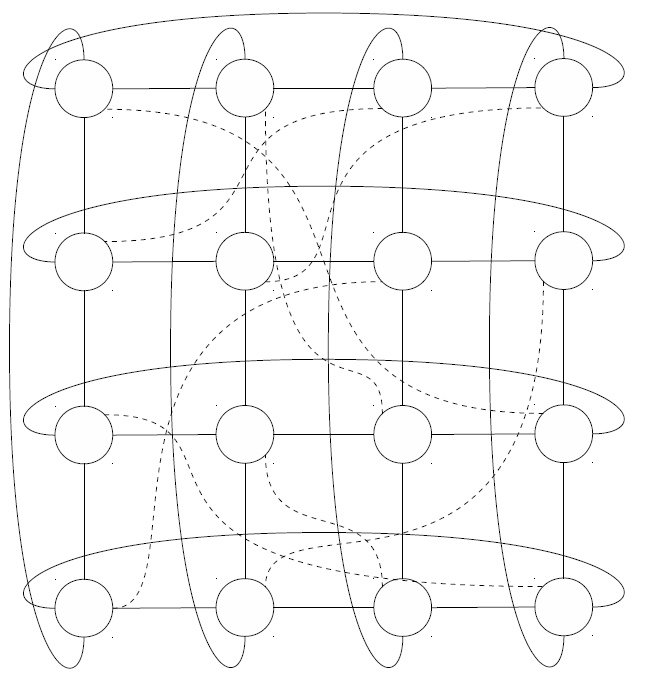
\includegraphics[width=.6\textwidth]{sw2d.png}
\caption{小世界网络\upcite{smallworld}}
\label{sw2d}
\end{figure}

\begin{figure}[htp]
\centering
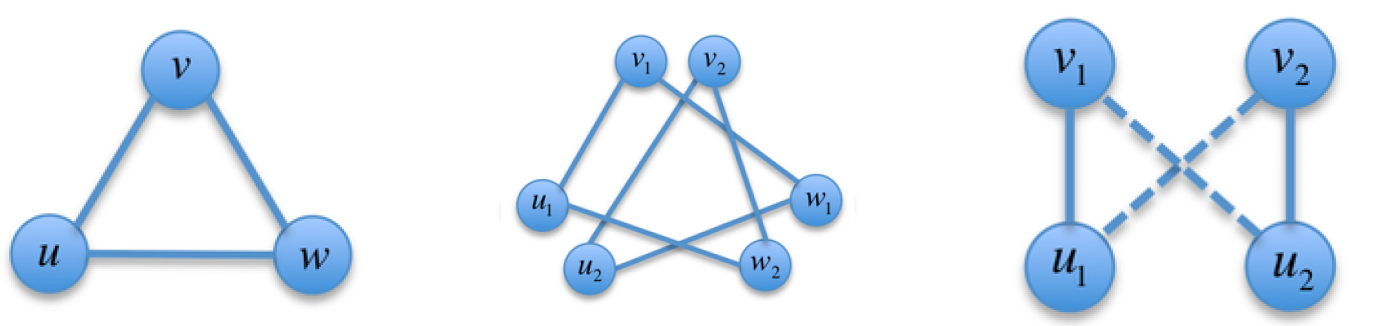
\includegraphics[width=.8\textwidth]{xpander.png}
\caption{Xpander结构\upcite{xpander}}
\label{xpander}
\end{figure}

Koibuchi等人\upcite{acaserandom}首先提出在高性能互连网络中采用随机拓扑结构
以满足系统延迟低、灵活扩展等需求。
具体构造方式类似于小世界网络的,在圆环拓扑结构上添加随机链路,
可以支持任意规模的网络。
在2013年的HPCA顶级会议上,
Koibuchi等人在之前提出的随机拓扑上进行了优化\upcite{layoutrandom},
加入了物理布局的考虑,限制了缆线的长度。
之后在2015年的IPDPS会议上他们研究组提出Skywalk拓扑结构\upcite{skywalk},
其进一步约束随机链路在实际物理布局的三维结构中的连接方式
来降低链路延迟对网络延迟的影响。
在2015年的HPCA顶级会议上,
他们研究组提出在机柜间利用基于自由空间光(FSO)的随机链路来
降低网络延迟并优化任务分配\upcite{fsorandom}。
如图\ref{fso}所示,通过在机柜上部署FSO设备,
以便根据任务负载添加FSO通信链路以优化性能。
随机拓扑虽然可以提供较短的网络直径和平均最短路径,
并可以灵活支持任意规模,
但是,路由算法是限制随机拓扑应用于实际系统部署的主要原因之一。
随机拓扑结构只能通过路由表的方式进行路由,
随着网络规模的增长,路由表规模呈指数级增长。

\begin{figure}[htp]
\centering
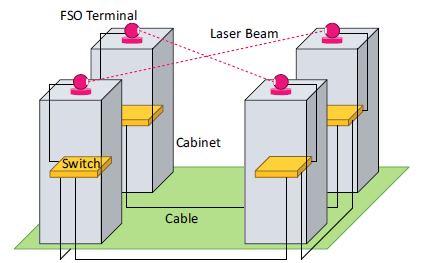
\includegraphics[width=.7\textwidth]{fso.png}
\caption{添加FSO链路的高性能互连网络\upcite{fsorandom}}
\label{fso}
\end{figure}

\section{高性能互连网络路由算法}

拓扑结构和路由算法是紧密相关的,路由算法决定了拓扑结构的实际网络性能。
路由算法除了决定报文在拓扑结构的路径也同时影响网络
在实际通信下的拥塞情况以及网络的死锁避免策略。
虽然在高性能互连网络中,新型拓扑的连接方式多种多样,
但是,相同点都是网络规模大且拓扑结构直径低。
这个相同点造成了新型拓扑结构只有少量的冗余最短路径和部分关键链路使用频率高,
如Slim Fly\upcite{slimfly}结构中只有
极少量的节点对之间有多余一条的最短路径,
如Dragonfly\upcite{dragonfly}结构中超级节点之间的链路会造成网络的拥塞。
在实际通信中,为了满足不同的应用负载,
使用自适应路由算法是提升网络性能、解决网络中链路拥塞的主要方法之一,
那么,在新型拓扑结构中只能使用非最短路径代替最短路径。
这不仅给自适应路由算法的性能带来挑战,
同时也给死锁避免策略带来成本开销和工艺设计等挑战。

Dragonfly结构是高性能互连网络的新型拓扑结构典型代表之一,
研究其结构特点提出的路由算法较多。

最短路径路由(MIN)是Dragonfly结构上最简单和最基本的路由算法\upcite{dragonfly}。
使用最短路径路由最多只需3跳就能将报文从源路由节点到目的路由节点,
即报文最多通过源路由节点所在的超级节点内的本地链路以及
源超级节点和目的超级节点的全局链路和目的超级节点的本地链路。
因为Dragonfly的结构特点,本地链路和全局链路的VC可以复用,
则MIN 至少需要两条VC来避免死锁。

非最短路径路由又称Valiant路由算法(VAL)\upcite{dragonfly},
是针对高负载流量提出的路由算法。
报文先选择一个中介节点作为第一个目的路由节点,
当通过MIN从源路由节点到达中介节点后再通过MIN 从中介节点到达目的路由节点。
这样做的好处是,缓解高负载流量对全局链路的过度请求。
具体在实施时Valiant路由算法可划分为两种,
一种是以中介节点所在的超级节点为第一目的地,
只要报文到达中介节点所在的超级节点就将目的地换成真正的目的路由节点。
第二种则是按前面介绍的以中介节点为第一目的地(VAL$_n$)\upcite{overcomefarend}。
第一种VAL最长需要经过5跳到达终点,途
经3条本地链路和2条全局链路。
VAL$_n$则最长需要经过6跳到达终点,途经3条本地链路和3条全局链路。
两种算法都至少需要3条VC来避免死锁。

根据网络状态选择走VAL机制或是MIN机制是均衡全局自适应路由算法
(UGAL)的主要机制\upcite{dragonfly}。
网络状态则由路由端口缓冲区队列长度和报文的跳步数共同决定。
在均衡随机通信模式下,VAL相比MIN,不仅跳步数翻倍,
吞吐率也会相应减半。而在密集高负载的最差通信模式下,
MIN则会造成全局链路的严重堵塞。
UGAL最长跳步数由VAL机制决定,
因此,至少需要3条VC来避免死锁。

上述四种Dragonfly结构路由算法并不能及时感知并反馈全局链路的拥塞,
因此,有研究提出间接自适应路由算法\upcite{indirect}来迅速对全局链路的拥塞作出反馈。
第一种间接自适应路由算法CRT (Credit Round Trip),
如图\ref{dragonflyir} 所示,
通过感知本地链路的信用反馈延迟来判断全局链路拥塞情况使得UGAL算法及时对拥塞做出
反馈,如路由器R0通过本地链路给路由器R1发送报文再通过全局链路给路由器R2发送报文,
路由器R1给路由器R0的信用反馈需等到路由器R2的信用反馈返回到R1才能发送。
CRT通过背压的方式获得全局链路的拥塞信号,
但是可能会造成本地链路拥塞。
第二种间接自适应路由算法PAR(Progressive Adaptive Routing),
如图\ref{dragonflyir}所示,在源超级节点通过当前
拥塞情况作出路由决策,选择MIN或者VAL。
这种方法在发现全局链路拥塞时不会将拥塞情况反馈给源路由器。
该算法会多走一跳本地链路,在使用VC隔离的方法来避免死锁时,需要多一条VC。
PAR可以扩展到在经过的每一个超级节点内部都根据当前网络状态选择MIN或者VAL。
第三种间接路由算法PB(Piggyback),
如图\ref{dragonflyir}所示,
通过给相邻节点广播全局链路的拥塞状态作出路由选择。
具体实现则需要在每个报文上都需要一个记录链路状态的向量位。
每个路由器都需要维护同一个超级节点内全局链路的状态信息。
该算法缺点是路由器维护全局链路拥塞信息的更新。
第四种间接路由算法RES(Reservation),
如图\ref{dragonflyir}所示,该方法是报文提前预约全局链路的资源,
如果预约成功则执行MIN路由,不成功则执行VAL路由。
该方法可能会造成预约信息泛滥以及预约信息不及时。

\begin{figure}[htp]
  \centering
    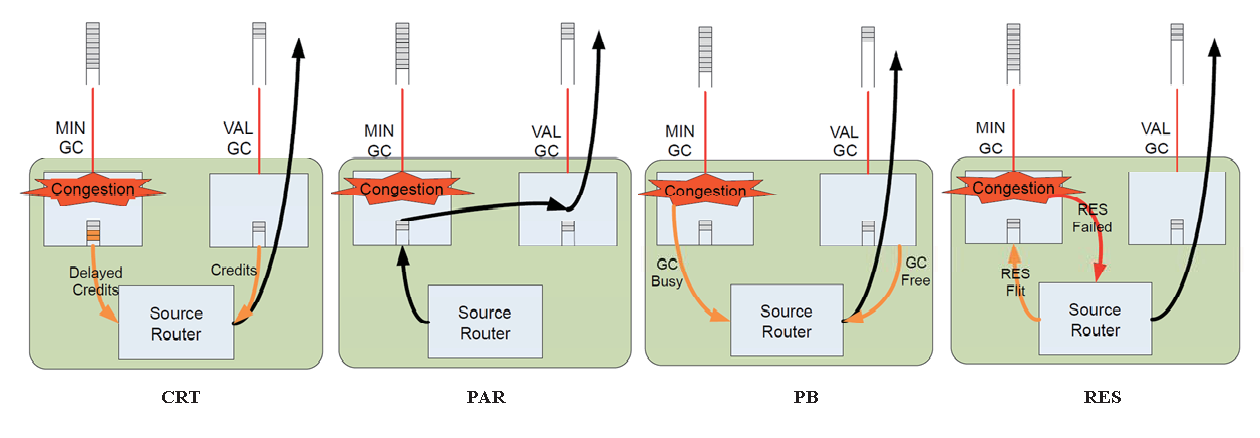
\includegraphics[width=.8\textwidth]{Visio-dragonfly_indirect.eps}
    \caption{Dragonfly结构间接自适应路由算法\upcite{indirect}}
       \label{dragonflyir}
\end{figure}

针对一些特定的通信负载,如最差通信负载,
Dragonfly结构中确定的两个超级节点频繁通信,
不仅造成全局链路拥塞,还会影响本地链路拥塞。
如图\ref{dragonflytr}所示,
在采用了VAL的路由选择后仍然会造成同一个超级节点的
两个路由器因为要转发所连接全局链路传送来的报文导致两个路由器之间的本地链路拥塞。
因此,研究者提出On-the-Fly 自适应路由算法(OFAR)\upcite{On-the-Fly}
来解决本地链路和全局链路的拥塞问题。
因为允许在超级节点内部进行本地链路的绕路,
有效避免因为全局链路拥塞造成本地链路的拥塞。
OFAR最长路径长度要达到8跳,如果采用VC隔离的方式避免死锁则至少需要6条VC。
OFAR最初采用的是基于气泡流量控制的哈密尔顿环作为逃逸子网。
OFAR-CM\upcite{OFAR-CM}则在OFAR 的基础上提出拥塞管理机制ECM和BCM,
这两种拥塞控制机制分别关注的是逃逸子网的拥塞情况和正常网络的拥塞情况,
并提出采用树型逃逸子网和up-down路由算法。

\begin{figure}[htp]
  \centering
    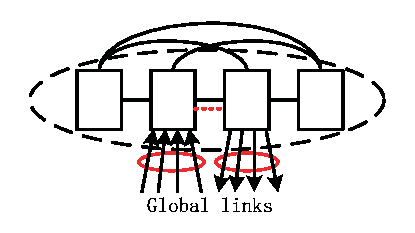
\includegraphics[width=.45\textwidth]{Visio-dragonfly_traffic.eps}
    \caption{Dragonfly结构中全局链路导致本地链路拥塞}
       \label{dragonflytr}
\end{figure}

为了避免死锁,有多种方法,大致可以分为三类:
一是设计无环路由,二是通过虚拟通道(VC)切换的方式避免死锁,
三是通过逃逸子网的方式避免死锁。
无环路由虽然是最经济的方法,但是会因为限制了部分路径不能通行,降低网络吞吐率。
VC 切换的方法虽然是可以充分利用网络中的链路,
但是VC数量的增加给工艺和成本开销带来挑战。
逃逸子网会使用一套独立的VC网络或者
物理网络执行一个没有环路的路由算法来避免整个网络的死锁,
相比前两种方法,逃逸子网可以算是一个折中的办法,
但是逃逸子网的使用频率影响网络性能。
RLM 和OLM算法\upcite{Rlmolm}的提出有效降低了OFAR对VC的需求。
RLM在超级节点内部采用转弯模型的方式即超级节点内部采用无环路由避免死锁,
通过减少路径多样性降低VC数量。
OLM则是采用限制VC使用顺序的方式避免死锁,
利用VC降序作为逃逸路径,
在保证超级节点内的路径多样性的同时不额外增加VC数量。

除了考虑不同的通信负载和拓扑结构的特征,
还有考虑实际物理布局中缆线长短对路由算法决策的影响。
在\upcite{overcomefarend}中指出目前大多数
已有的工作都没有考虑远端延迟的影响即下几跳后的网络拥塞和因路由器之间
较长链路延迟高引起的拥塞,实际上这些拥塞都只是暂时性的拥塞,
不会导致网络真正拥塞。
比如,较长的链路延迟会使得一些报文或者信用不能及时到达终点从而造成拥塞的假象。
因此,作者通过历史窗口的方法来避免这种假象影响自适应路由的决策
\upcite{overcomefarend}。

另外,如何分配缓冲区资源也对路由算法的性能有影响。
如Gorgues等人\upcite{Achieving}提出在$k-ary$ $n-cube$结构的片上网络上,
通过报文标记的方法给报文均衡分配网络中的缓冲区资源并利用更少的资源来避免死锁。
具体设计是每个输入端口有2条VC,
每条VC被分配一个报文长度的缓冲区大小。
完全自适应路由算法通过通过一条逃逸路径来避免死锁。
每次路由决策都可能改变报文的标记,
如果报文的决策是按维序路由算法路由的话就被标记为安全报文。
如果报文的决策不是按照维序路由算法路由的则被标记为不安全报文。
每个端口的两条VC中至少有一条VC里全是安全报文或者为空。
我们考虑将这种方法运用在片间网络上,不仅避免工艺上的挑战又能充分利用网络资源。

Head-of-Line Blocking(HoLB)问题也是影响路由算法性能的重要因素。
HoLB问题就是位于队列头的报文因为下一级拥塞不能前进阻挡了队列中其他报文前进。
相比确定性路由算法,即在源节点已经确定好报文传输路径,
自适应路由算法因为路由的灵活性会造成报文传输路径不唯一,
更容易造成HoLB问题\upcite{holbara}。
有研究组针对不同拓扑结构路由算法的HoLB问题提出了解决办法。
如在\upcite{holbara}中,针对直接网络的自适应路由算法,
利用有限的VC,将不同目的节点的报文分配到不同的VC中传输。
在\upcite{bbq}\upcite{DBBM}\upcite{iodet}中,
都使用类似的方法解决HoLB问题。
另外,提出上述方法的研究组也针对Dragonfly结构、Slim Fly结构
等典型新型高性能互连网络拓扑结构的路由算法解决HoLB问题
\upcite{holbdf}\upcite{holbsf}。
在FlexVC\upcite{flexvc}中则是提出一个缓冲区管理策略来降低网络HoLB问题,
具体方法就是在保证无死锁的条件下,
尽可能的增大VC可选择的范围。
如针对Slim Fly结构,如果采用最短路径路由算法,
网络中有3条VC的时候,报文就可以选择Opportunistic路径进行路由来降低HoLB问题。

\section{高性能互连网络拥塞控制机制}
拥塞控制机制跟路由算法是影响高性能互连网络网络性能的重要因素。
由于高性能互连网络具备无损的特性,即不会因为网络拥塞而丢包,
传统的拥塞控制机制,如TCP协议,就不适用于高性能互连网络。
高性能互连网络中经典的拥塞控制机制,
如Explicit Congestion Notification(ECN)拥塞控制机制,
是一种被动的拥塞控制机制,根据缓冲队列长度,
给报文打标签,到达目的节点后将拥塞信息通过ACK报文告诉源节点。
这种策略最大的缺点就是不能及时对拥塞作出反馈,响应速度慢。
因此,在2012年国际顶级会议SC上,Jiang等人提出
Speculative Reservation Protocol (SRP)\upcite{srp}拥塞控制机制。
SRP是一种主动拥塞控制机制,
通过light-weight的终端预约机制以及投机报文传输机制有效缓解热点通信模式下的拥塞,
获得比ECN机制更高的吞吐率。
之后,该研究组在2013 年SC会议上提出
Channel Reservation Protocol(CRP)\upcite{crp}策略,
专门解决大规模无损网络通信时关键链路拥塞的问题。
因为考虑到成本和技术的限制,集群之间的链路都是供小于求,
如图\ref{crp}所示,如果热点H不能正常吸收负载则会造成,
数据流Z拥塞在点A,进而产生拥塞树,
不仅影响集群0的数据流Y还影响集群1内要到达点H的数据流。
CRP通过预约关键链路的方法来解决瓶颈链路。
在2015年的SC会议上,
该研究组针对ECN和SRP对small message终端拥塞反应速度慢和易造成
拥塞树等不足,
提出Small-Message SRP(SMSRP)和
Last-Hop Reservation Protocol (LHRP)两种策略\upcite{smsrp}。
相较于SRP策略,
SMSRP策略会在发送预约报文之前发送一些投机报文以免造成带宽浪费
以及因为预约产生的动荡。
LHRP相较于SRP和SMSRP策略不同的则是在最后一跳交换机处根据终端的缓冲队列长度对
投机报文传输失败作出反馈。

\begin{figure}[htp]
  \centering
    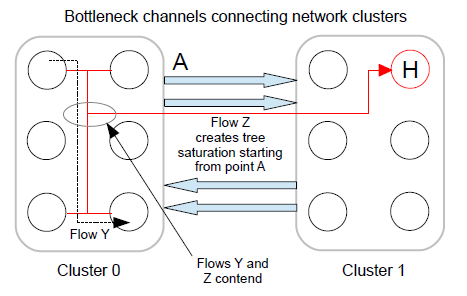
\includegraphics[width=.65\textwidth]{crp.png}
    \caption{集群间的拥塞树\upcite{crp}}
       \label{crp}
\end{figure}

除了上述基于预约的拥塞控制机制,Kim等人在2016年的国际顶级会议MICRO上
提出一种新的拥塞管理策略Contention-based Congestion Management(CBCM)
\upcite{cbcm}。在CBCM中指出,当网络中只采用自适应路由算法来提升网络性能的时候,
往往会造成拥塞扩散性能降低的情况。
自适应路由算法是用来解决网络拥塞,
即网络中的链路拥塞,而拥塞控制机制则是解决终端节点的超额订购。
当两者搭配使用才能更好的提升网络性能。
CBCM的原理如图\ref{cbcm}所示,CBCM专门使用一条额外的VC分离终端拥塞的影响,
一旦发现终端拥塞,即终端接收到被标记的报文超过阈值,
则节流相应的源节点且节流的报文在这额外的VC中采用最短路由算法,
为了避免因为自适应路由算法扩散拥塞。

\begin{figure}[htp]
  \centering
    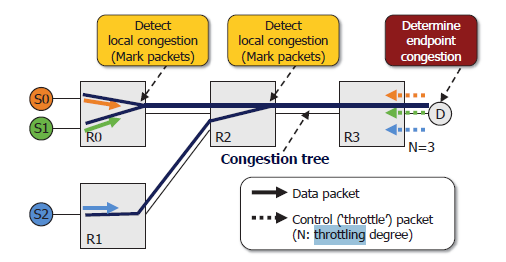
\includegraphics[width=.65\textwidth]{cbcm.png}
    \caption{Contention-based Congestion Management机制\upcite{cbcm}}
       \label{cbcm}
\end{figure}
%\section{模拟环境和性能测试平台}

\section{本章小结}
本章主要阐述了大规模低直径高性能互连网络的理论基础和相关研究。
主要综述了目前已提出的典型高性能互连网络的拓扑结构和典型路由算法等内容。
本文基于大规模低直径的特点开展高性能互连网络拓扑结构设计和路由算法的研究。
